%------------------------------------------------------------------------------
% Code
%------------------------------------------------------------------------------

\input{assets/code/names}
\input{assets/misc/posterHelpers}

% for assets/code/example.tex...
\newcommand{\exampleCode}{\input{assets/code/example}}
\newcommand{\refExampleCode}{\Cref{lst:exampleCode}}

% for assets/code/examplePseudocode.tex...
\newcommand{\examplePseudocode}{\input{assets/code/examplePseudocode}}
\newcommand{\refExamplePseudocode}{\Cref{lst:examplePseudocode}}

% for assets/code/mainInvalidInputTest.tex...
\newcommand{\mainInvalidInputTest}{\input{assets/code/mainInvalidInputTest}}
\newcommand{\refMainInvalidInputTest}{\Cref{lst:mainInvalidInputTest}}

% for assets/code/projManualViolationReq.tex...
\newcommand{\projManualViolationReq}{\input{assets/code/projManualViolationReq}}
\newcommand{\refProjManualViolationReq}{\Cref{lst:projManualViolationReq}}

% for assets/code/projViolationChoice.tex...
\newcommand{\projViolationChoice}{\input{assets/code/projViolationChoice}}
\newcommand{\refProjViolationChoice}{\Cref{lst:projViolationChoice}}

%------------------------------------------------------------------------------
% Graphs
%------------------------------------------------------------------------------

% Organization of files

\newcommand{\parChdGraphs}{
    % Only top or bottom to comply with IEEE guidelines
    \begin{figure}[b!]
        \centering
        \begin{subfigure}[b]{\linewidth}
            \centering
            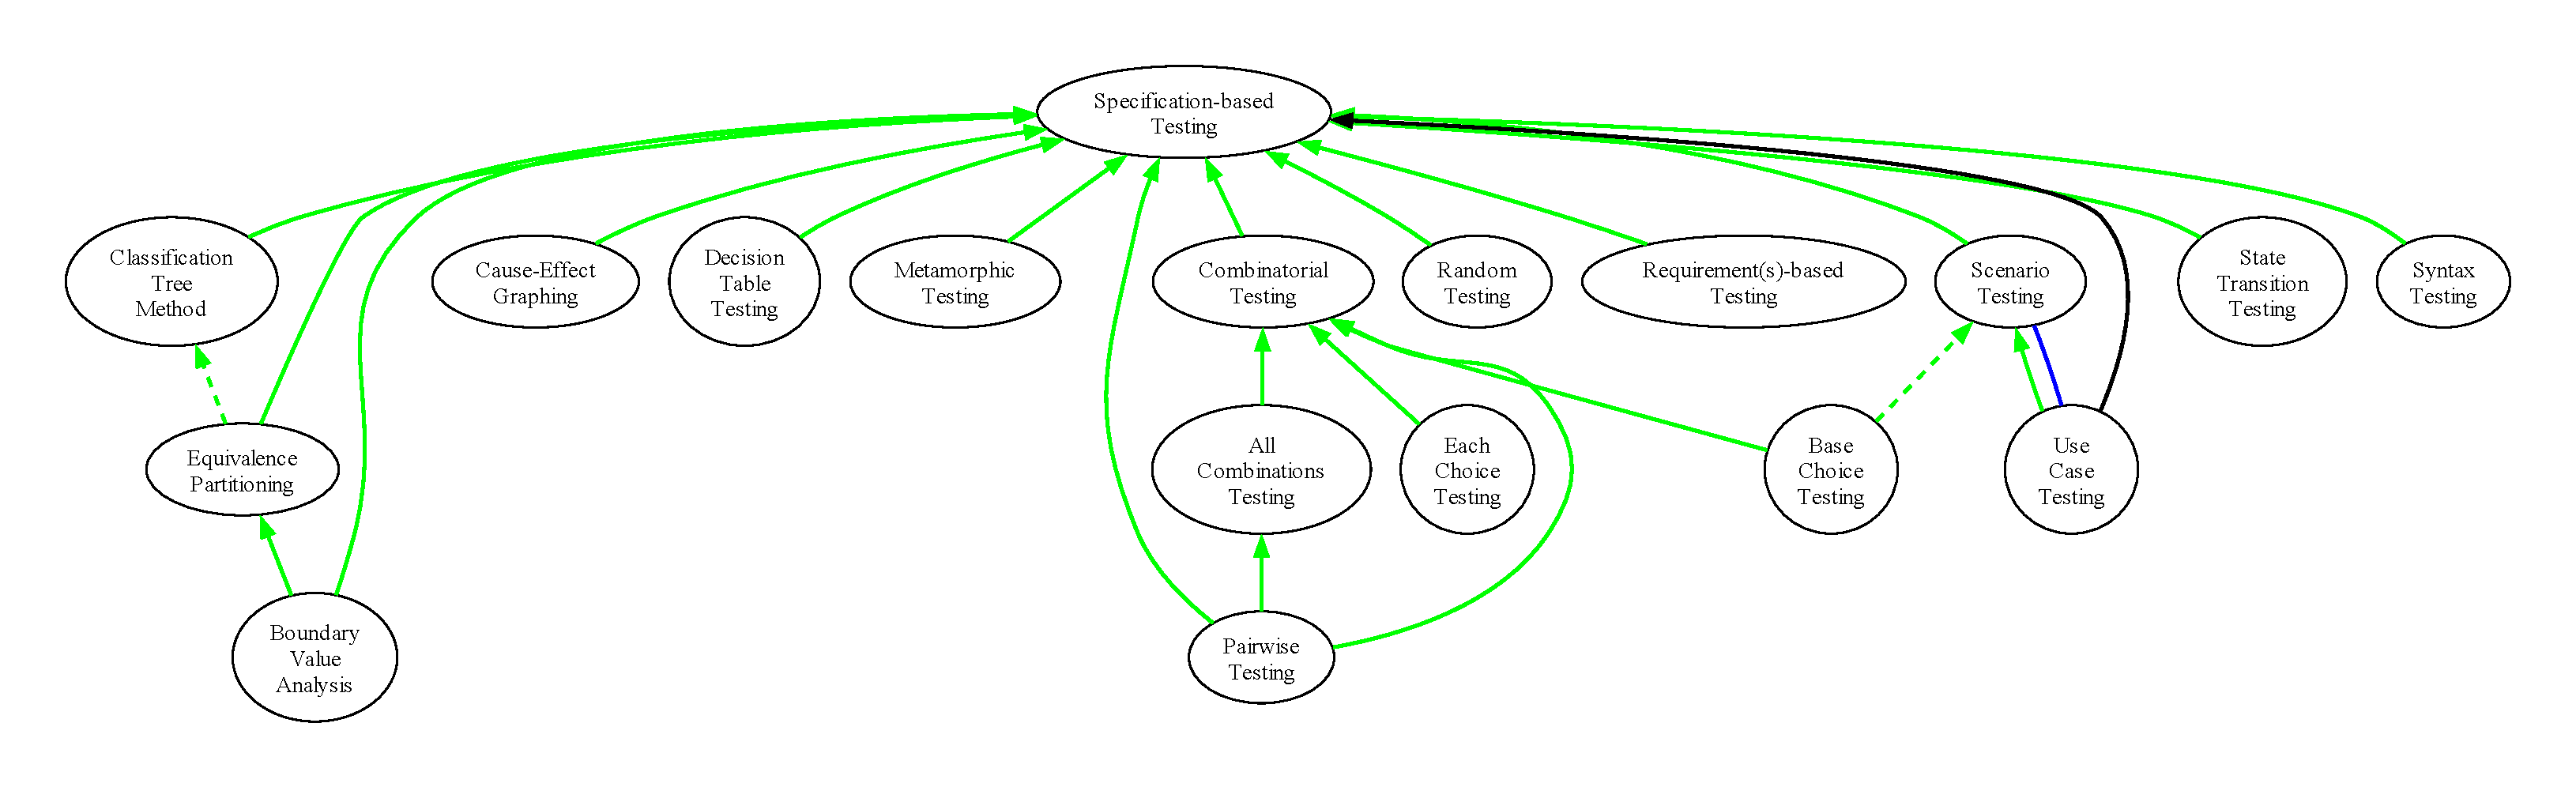
\includegraphics[width=\linewidth]{assets/graphs/specBasedGraph.pdf}
            \caption{``Superset'' relations.}
            \label{fig:specBasedGraph}
        \end{subfigure}
        \begin{subfigure}[t]{.45\linewidth}
            \centering
            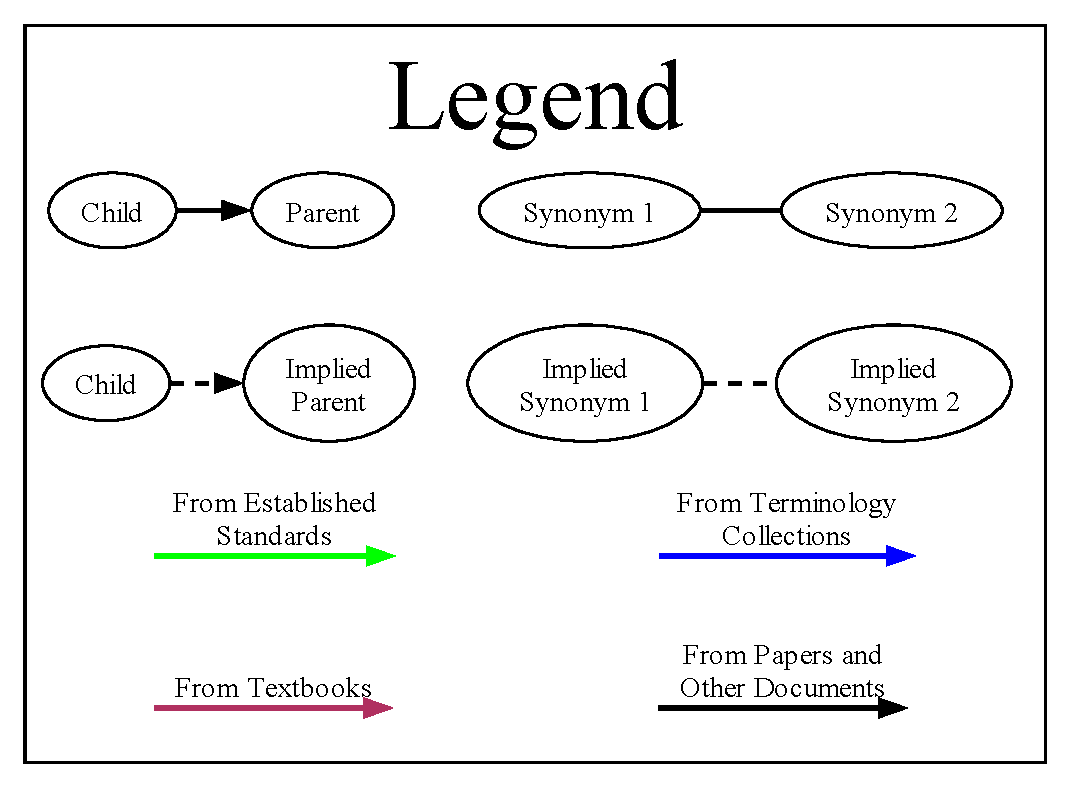
\includegraphics[width=\linewidth]{assets/graphs/parChdLegend.pdf}
        \end{subfigure}
        \begin{subfigure}[t]{.5\linewidth}
            \centering
            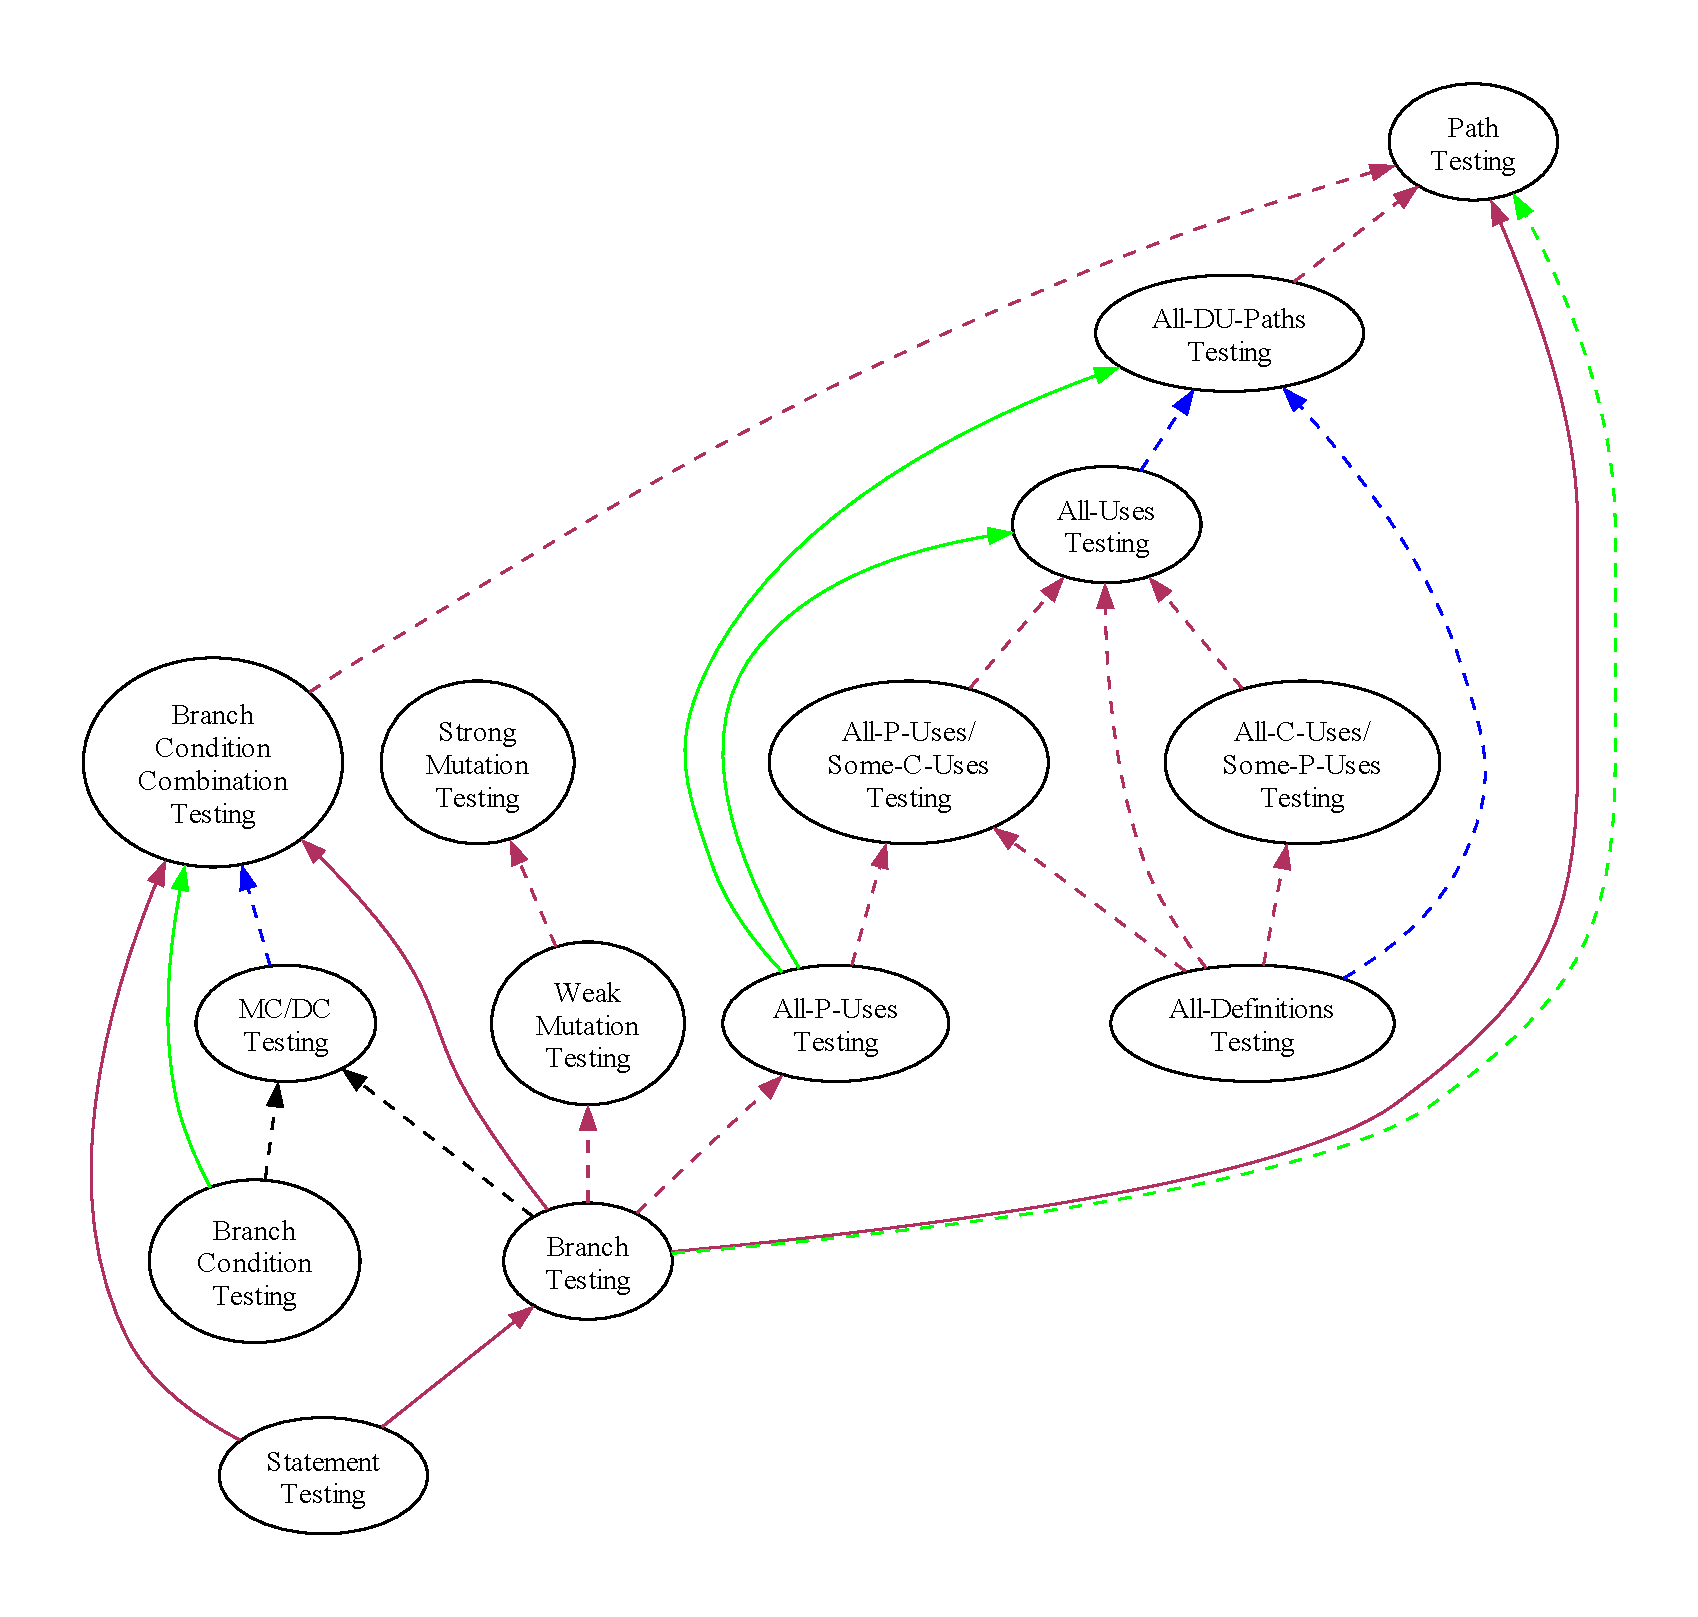
\includegraphics[width=\linewidth]{assets/graphs/subsumesGraph.pdf}
            \caption{``Subsume'' relations.}
            \label{fig:subsumesGraph}
        \end{subfigure}
        \caption{Graphs of different classes of parent-child relations.}
        \label{fig:parChdGraphs}
    \end{figure}
}

\newcommand{\ExampleGraph}{
    \begin{figure*}
        \begin{subfigure}[b]{0.275\linewidth}
            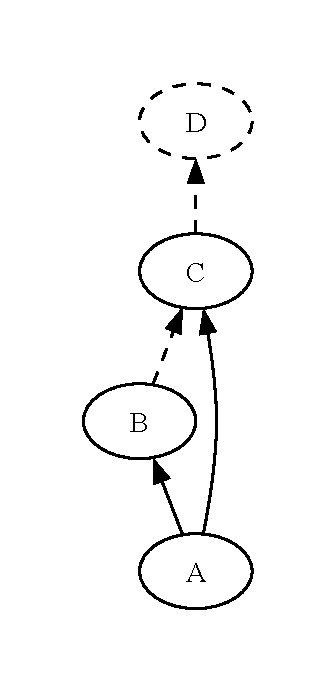
\includegraphics[width=\linewidth]{assets/graphs/ExampleGlossaryGraph.pdf}
            \caption{Graph from \\ \Cref{tab:exampleGlossary}.}
            \label{fig:exampleGraph}
        \end{subfigure}
        \centering
        \begin{subfigure}[b]{0.7\linewidth}
            \centering
            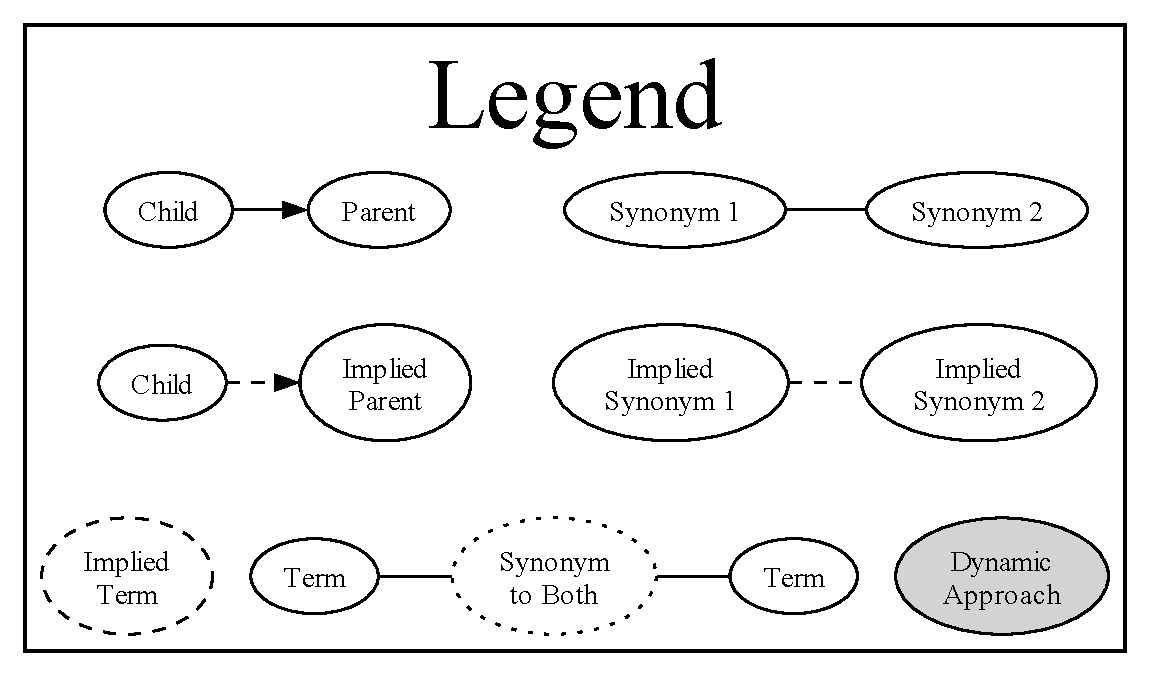
\includegraphics[width=\linewidth]{assets/graphs/manual/manualLegend.pdf}
            \hspace{5cm}\begin{subfigure}[t]{0.475\linewidth}
                \includegraphics[width=1.1\linewidth]{assets/graphs/rigidExampleGlossaryGraph.pdf}
                \caption{Rigid graph from\\\Cref{tab:exampleGlossary}.}
                \label{fig:rigidExampleGraph}
            \end{subfigure}
            \begin{subfigure}[t]{0.475\linewidth}
                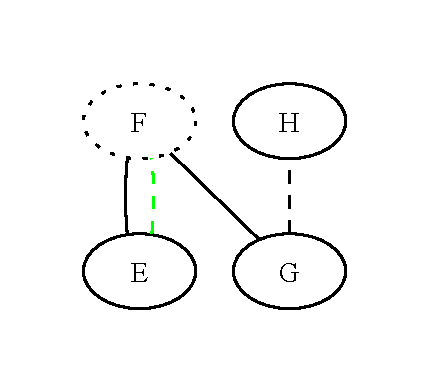
\includegraphics[width=1.1\linewidth]{assets/graphs/SynExampleGlossaryGraph.pdf}
                \caption{Graph from \Cref{tab:synExampleGlossary}.}
                \label{fig:synExampleGraph}
            \end{subfigure}
        \end{subfigure}
        \begin{subfigure}[t]{0.25\linewidth}
            \centering
            \includegraphics[width=1.2\linewidth]{assets/graphs/SelfExampleGlossaryGraph.pdf}
            \caption{Self-loop graph.}
            \label{fig:selfExampleGraph}
        \end{subfigure}
        \hfill
        \begin{subfigure}[t]{0.425\linewidth}
            \centering
            \includegraphics[width=0.6\linewidth]{assets/graphs/ParSynExampleGlossaryGraph.pdf}
            \caption{Graph of a pair of terms with a \hyperref[par-chd-rels]{parent-child} \emph{and} synonym relation.}
            \label{fig:parSynExampleGraph}
        \end{subfigure}
        \hfill
        \begin{subfigure}[t]{0.25\linewidth}
            \centering
            \includegraphics[width=1.4\linewidth]{assets/graphs/StaticExampleGlossaryGraph.pdf}
            \caption{Static graph.}
            \label{fig:staticExampleGraph}
        \end{subfigure}
        \caption{Example generated graphs.}
        \label{fig:exampleGraphs}
    \end{figure*}
}

\newcommand{\recoveryGraphs}{
    % Only top or bottom to comply with IEEE guidelines
    \begin{figure}[bt!]
        \centering
        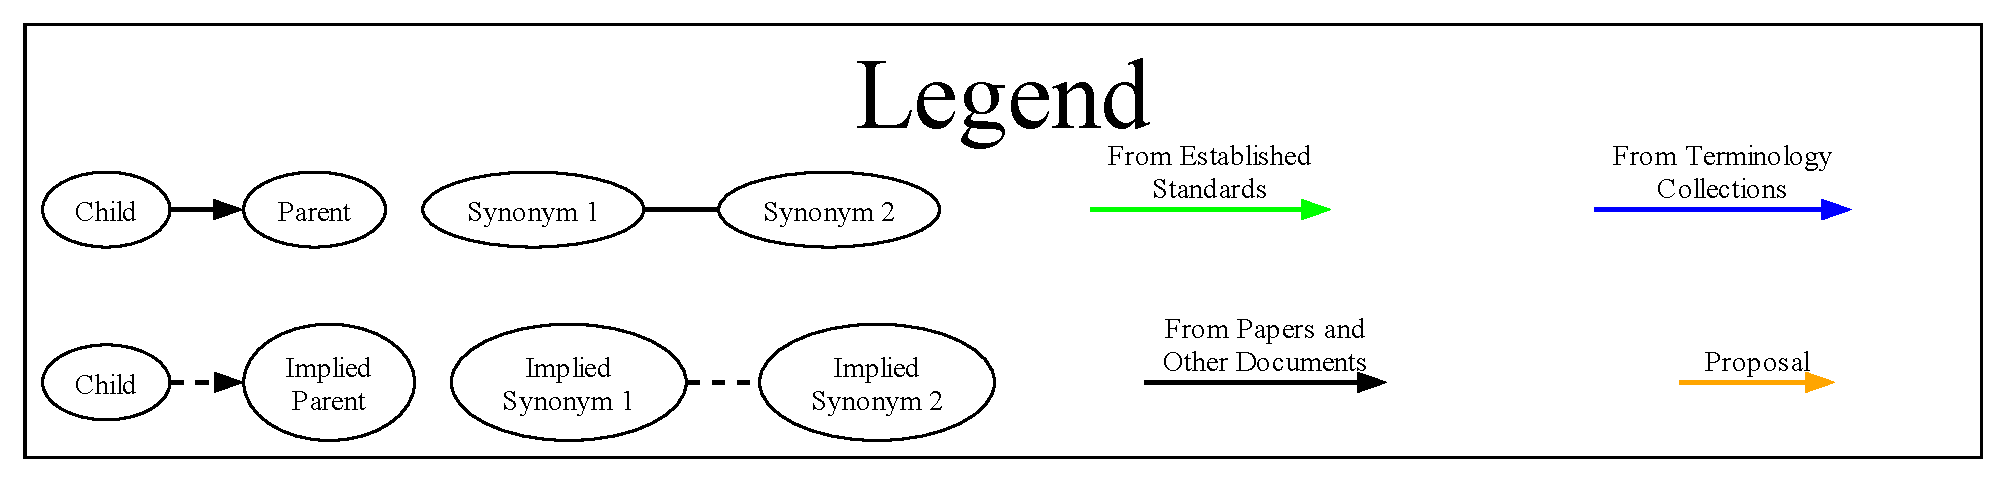
\includegraphics[width=\linewidth]{assets/graphs/recoveryLegend.pdf}
        \begin{subfigure}[b]{.475\linewidth}
            \centering
            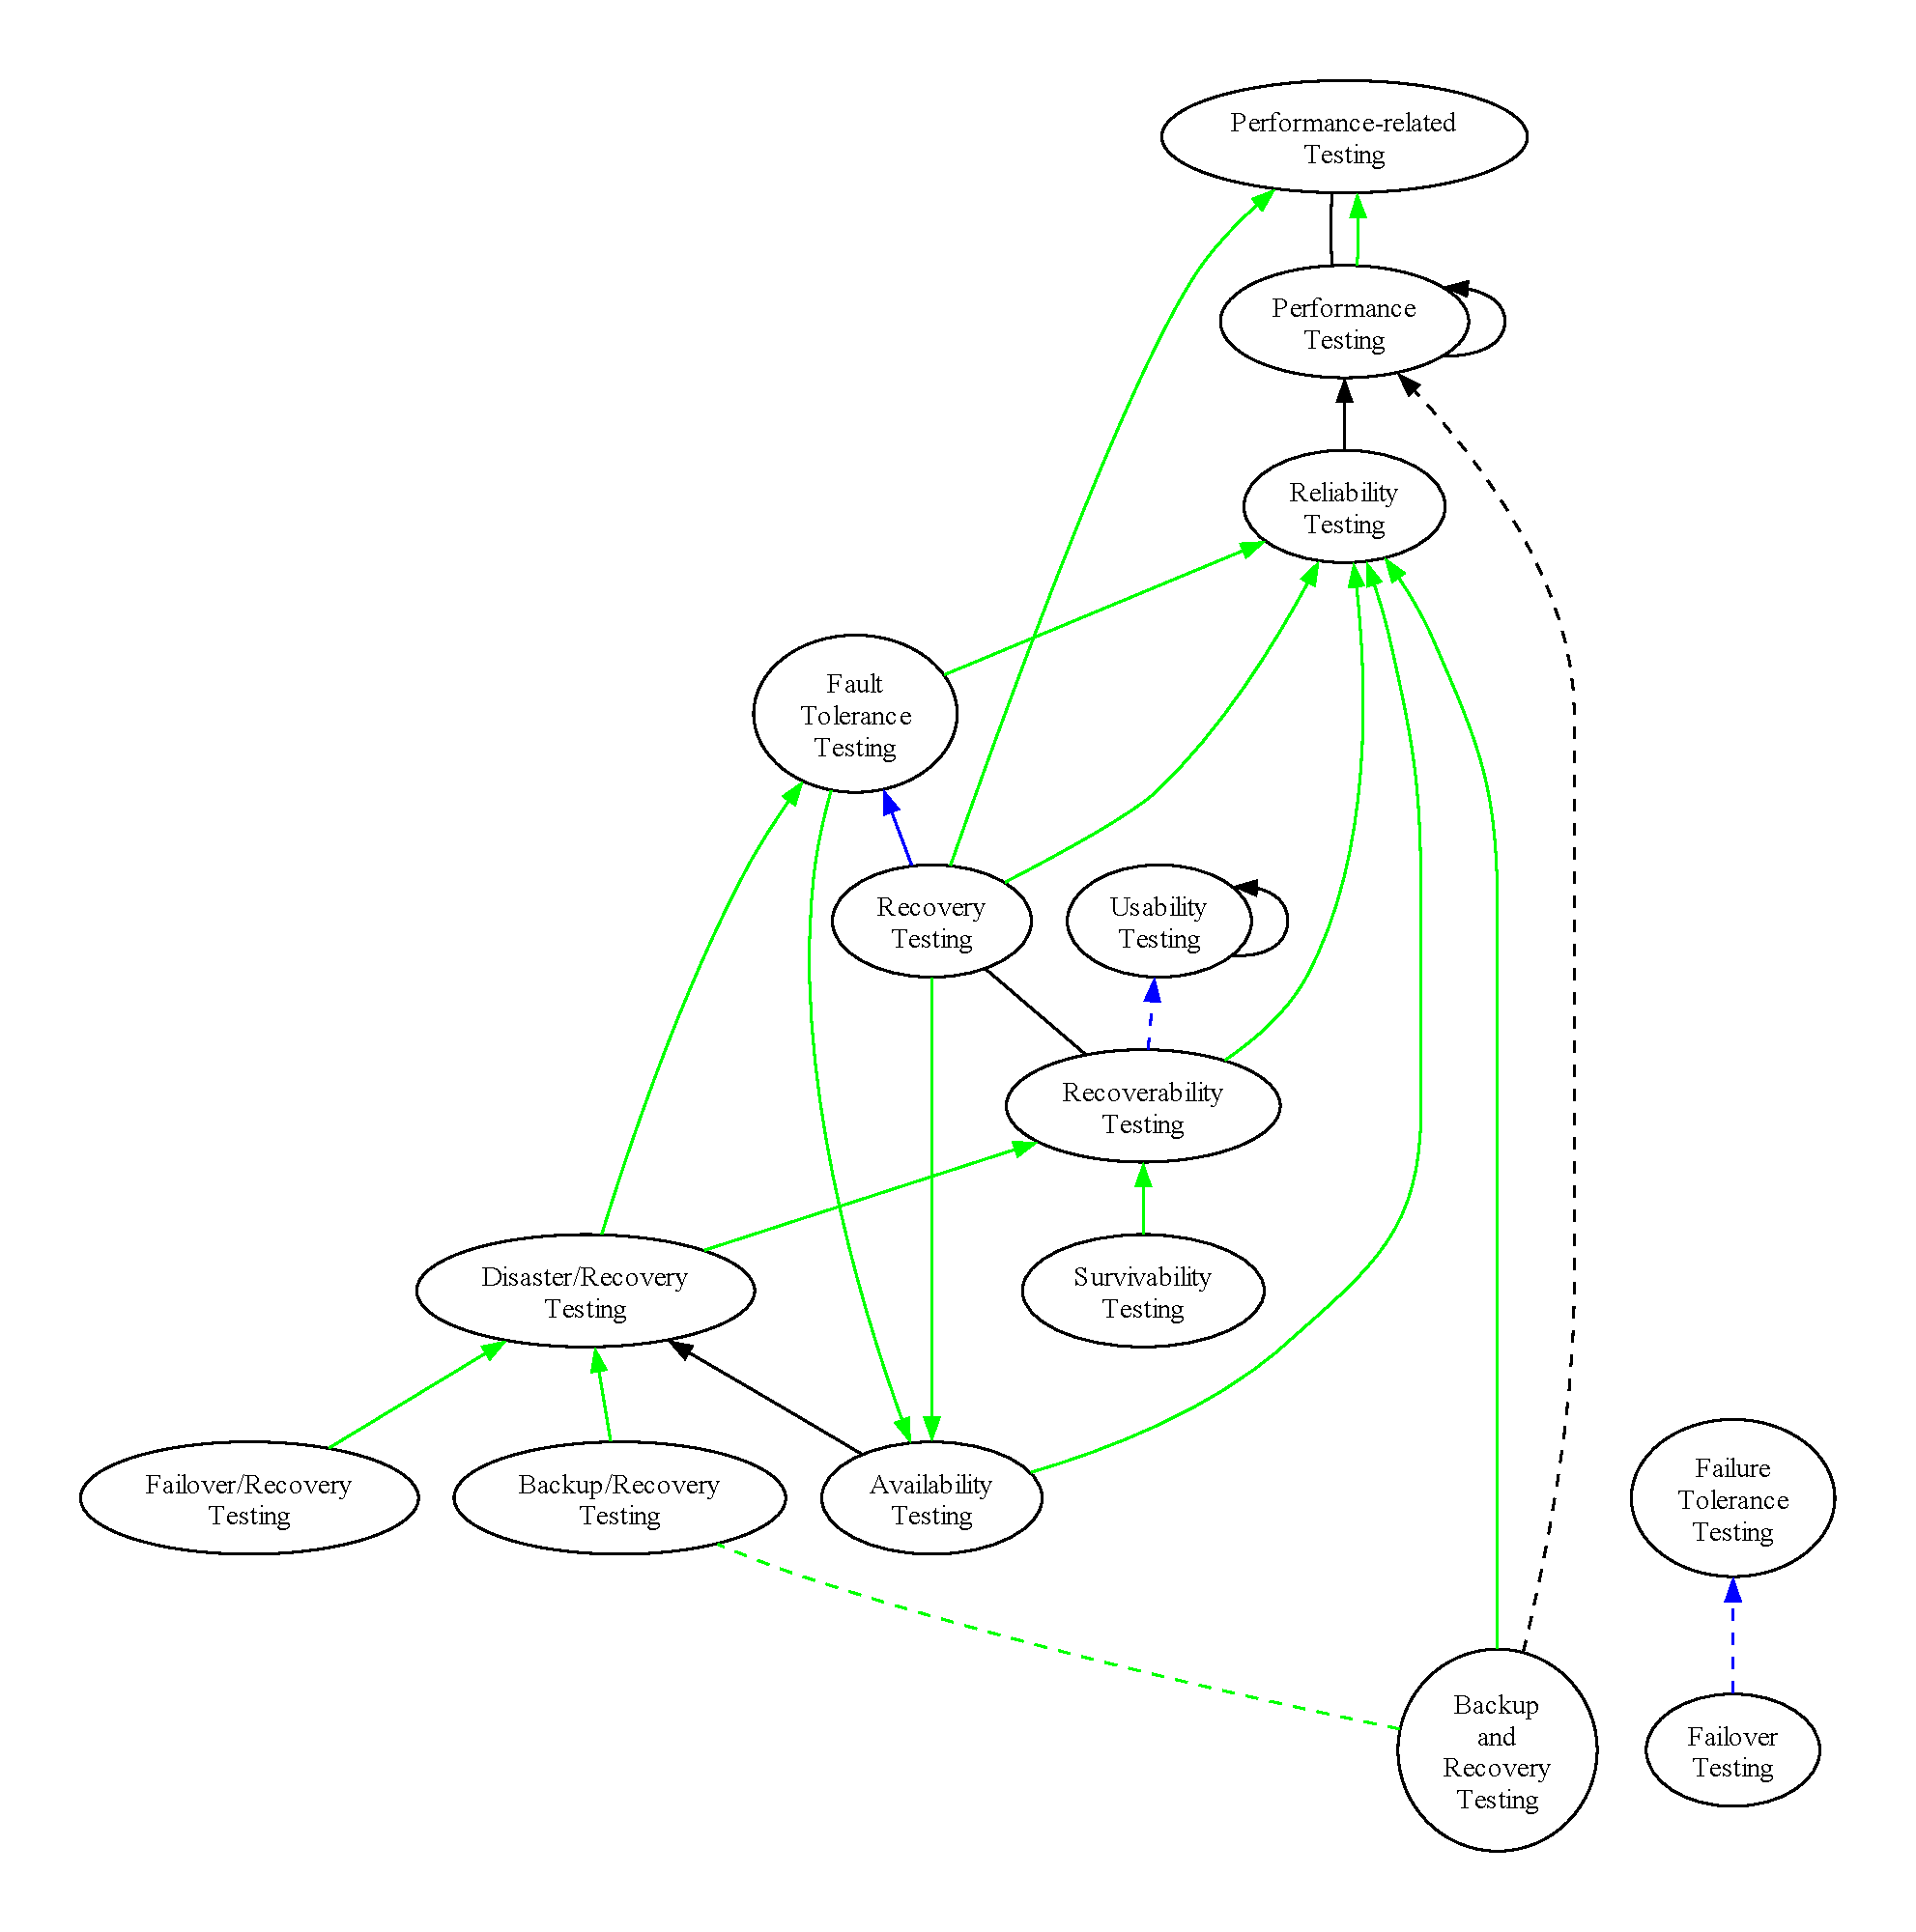
\includegraphics[width=\linewidth]{assets/graphs/recoveryGraph.pdf}
            \caption{Graph of current relations.}
            \label{fig:rec-graph-current}
        \end{subfigure}
        \begin{subfigure}[b]{.475\linewidth}
            \centering
            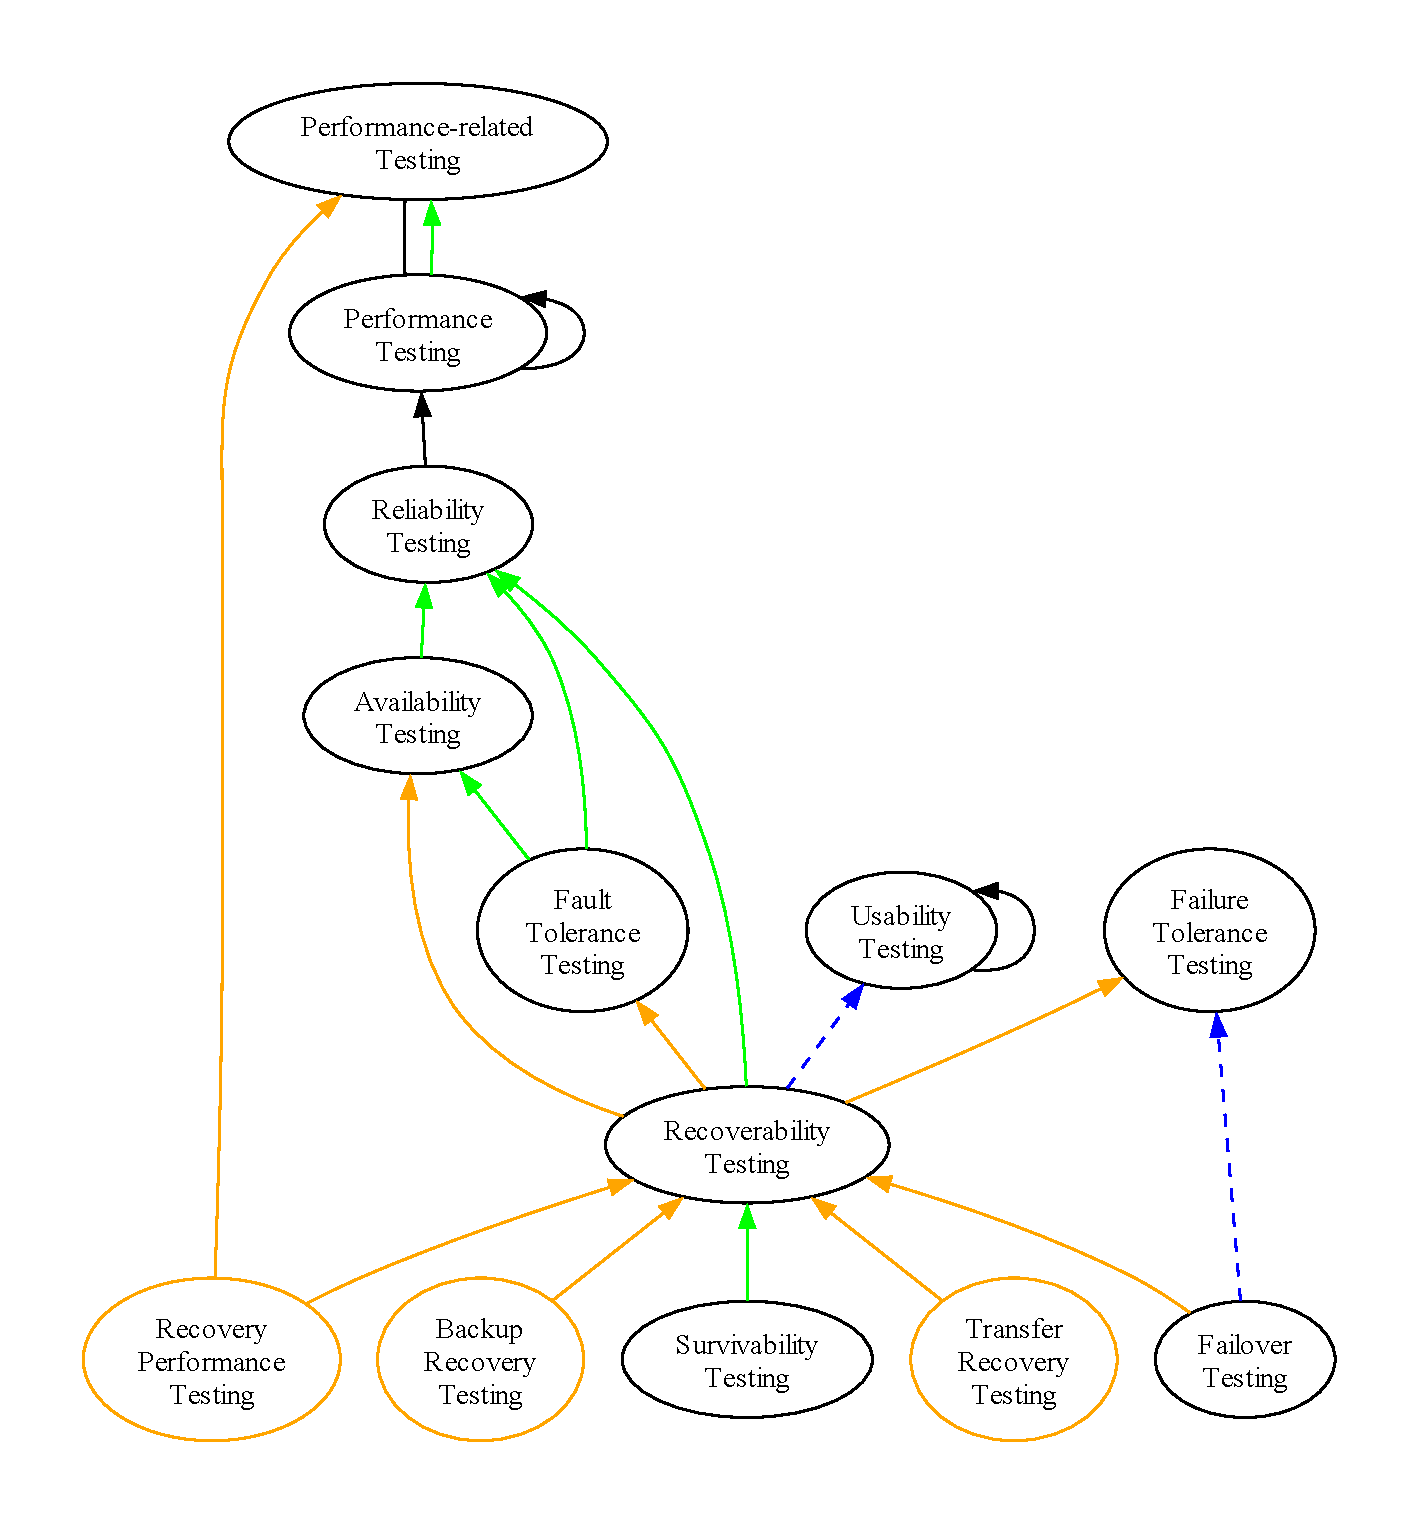
\includegraphics[width=\linewidth]{assets/graphs/recoveryProposedGraph.pdf}
            \caption{Graph of proposed relations.}
            \label{fig:rec-graph-proposed}
        \end{subfigure}
        \caption{Graphs of relations between terms related to recovery testing.}
        \label{fig:recoveryGraphs}
    \end{figure}
}

\newcommand{\scalGraphs}{
    % Only top or bottom to comply with IEEE guidelines
    \begin{figure}[b!]
        \centering
        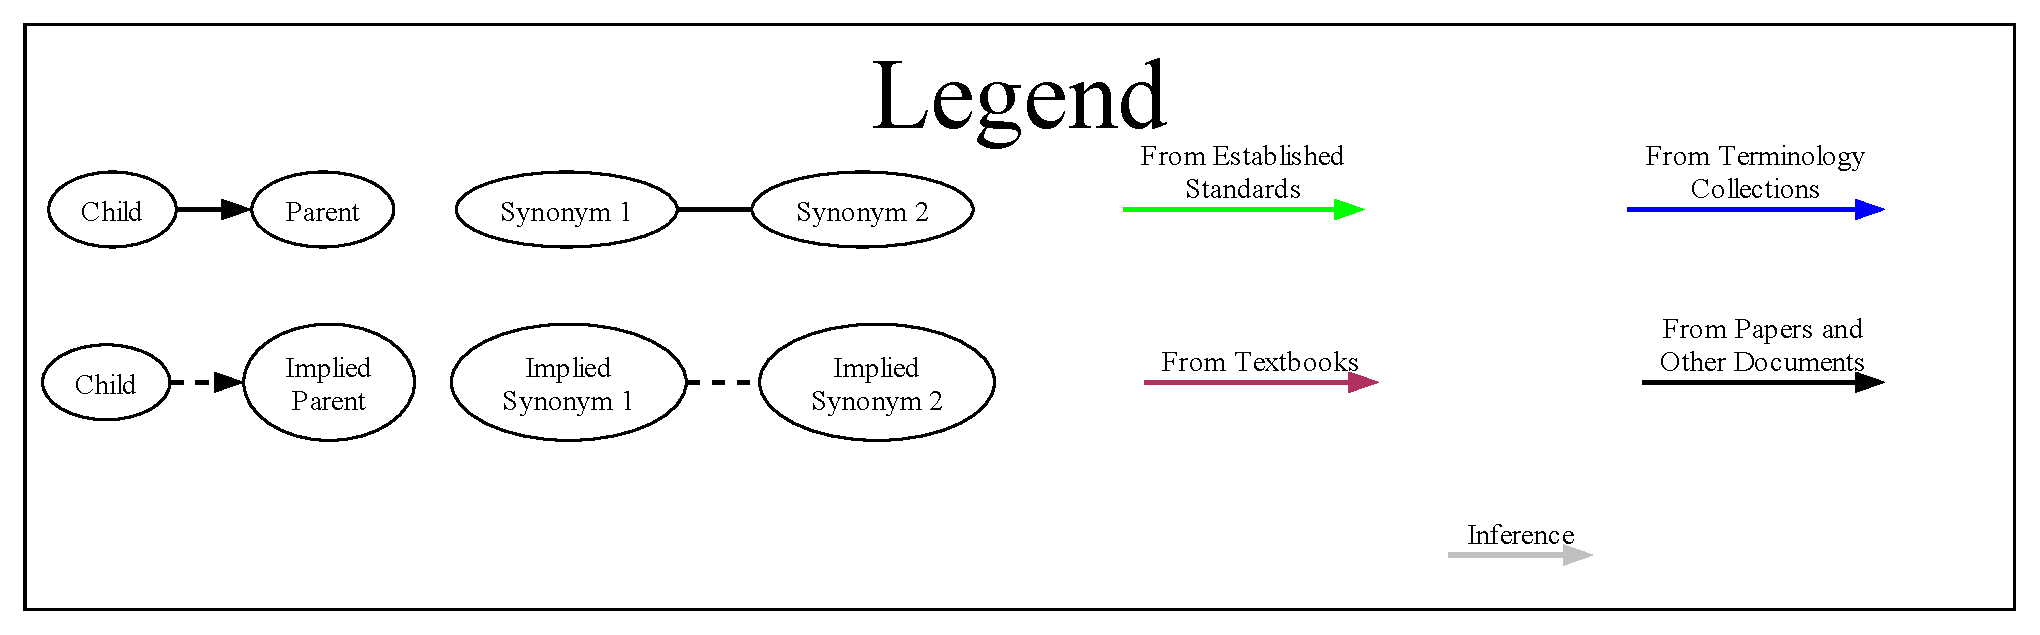
\includegraphics[width=\linewidth]{assets/graphs/scalabilityLegend.pdf}
        \begin{subfigure}[b]{.475\linewidth}
            \centering
            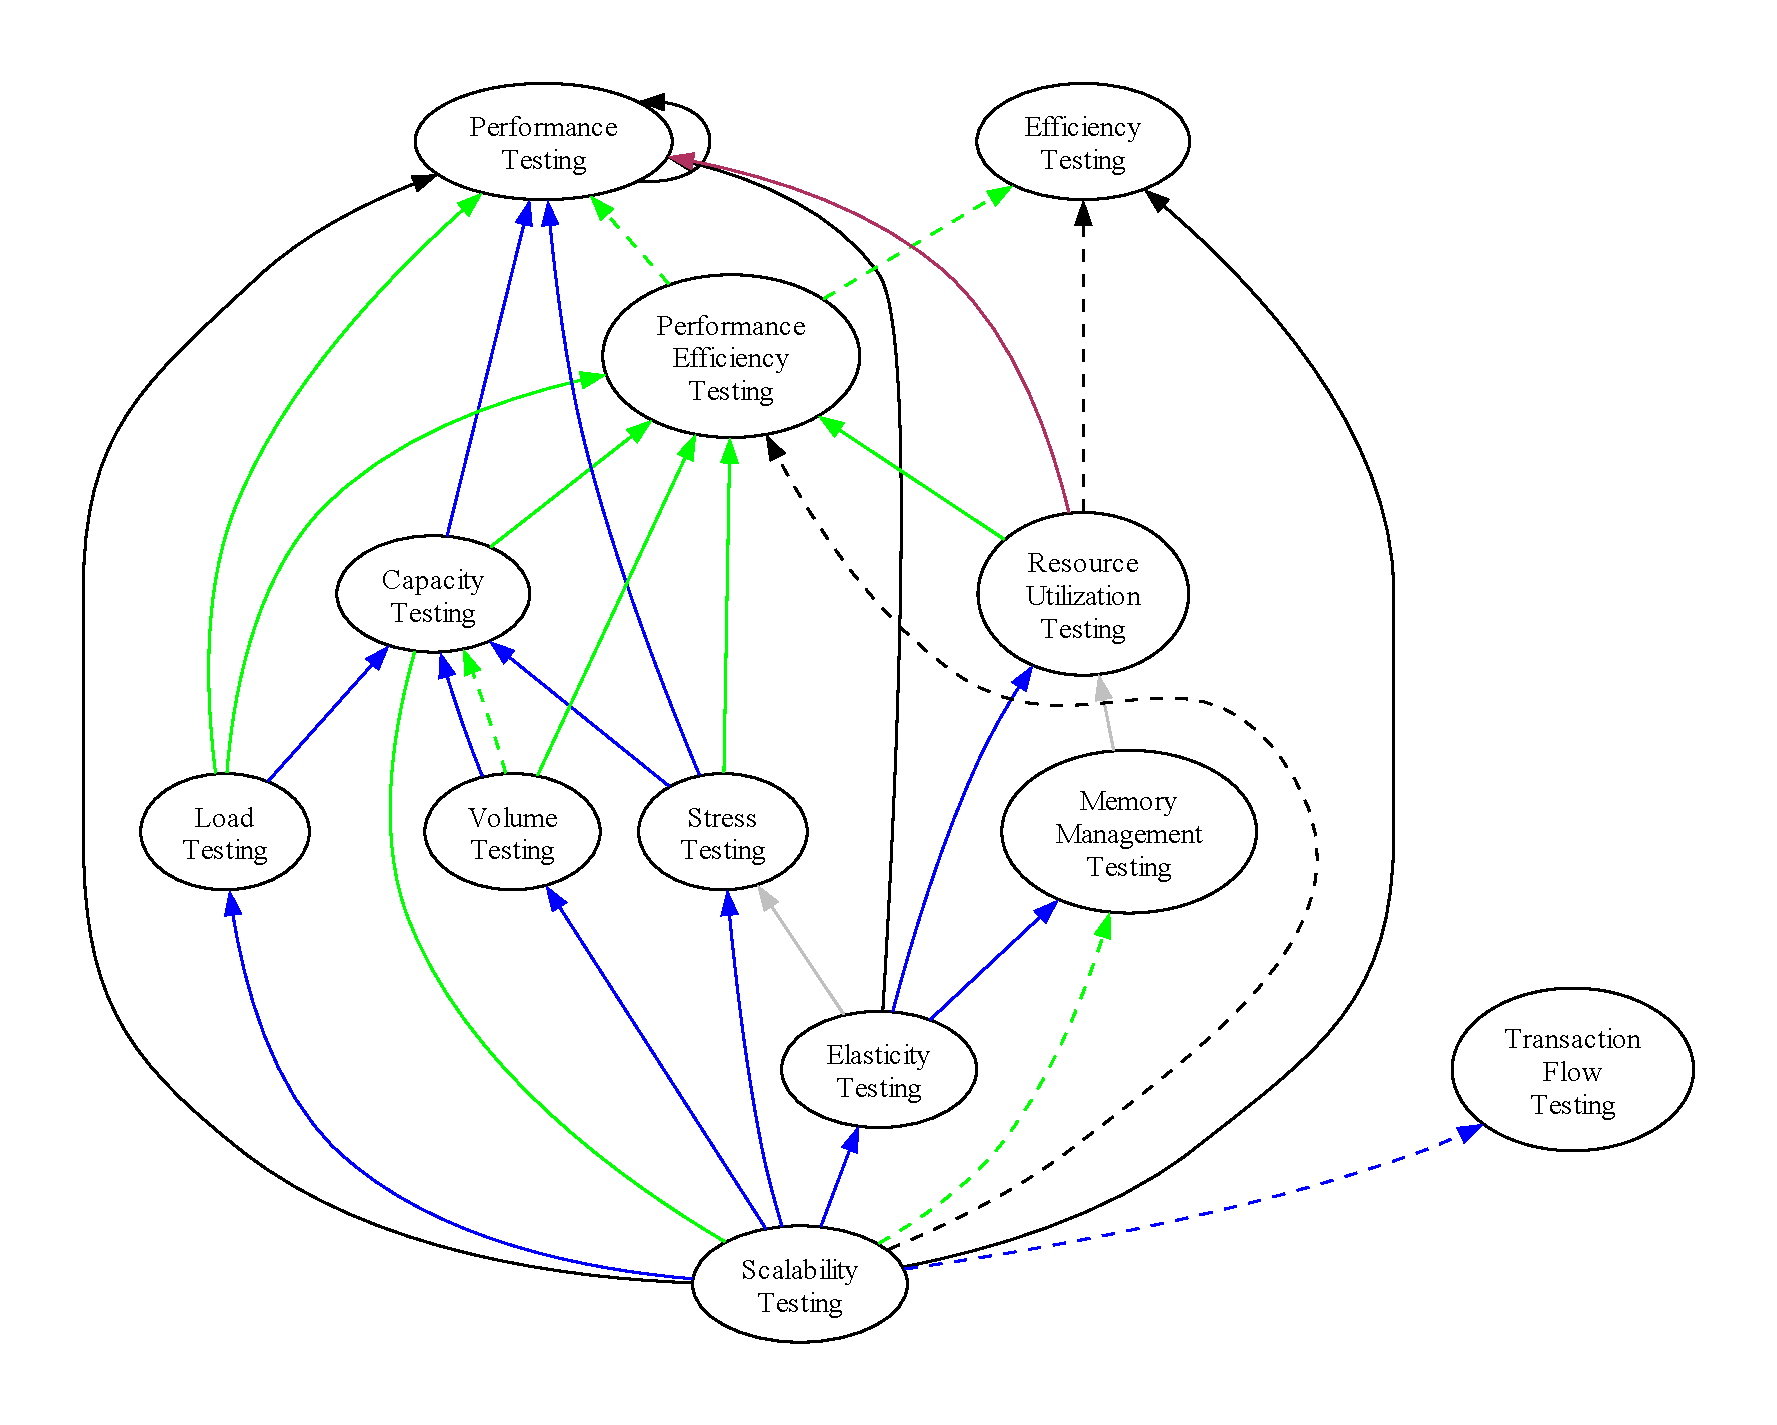
\includegraphics[width=\linewidth]{assets/graphs/scalabilityGraph.pdf}
            \caption{Graph of current relations.}
            \label{fig:scal-graph-current}
        \end{subfigure}
        \begin{subfigure}[b]{.475\linewidth}
            \centering
            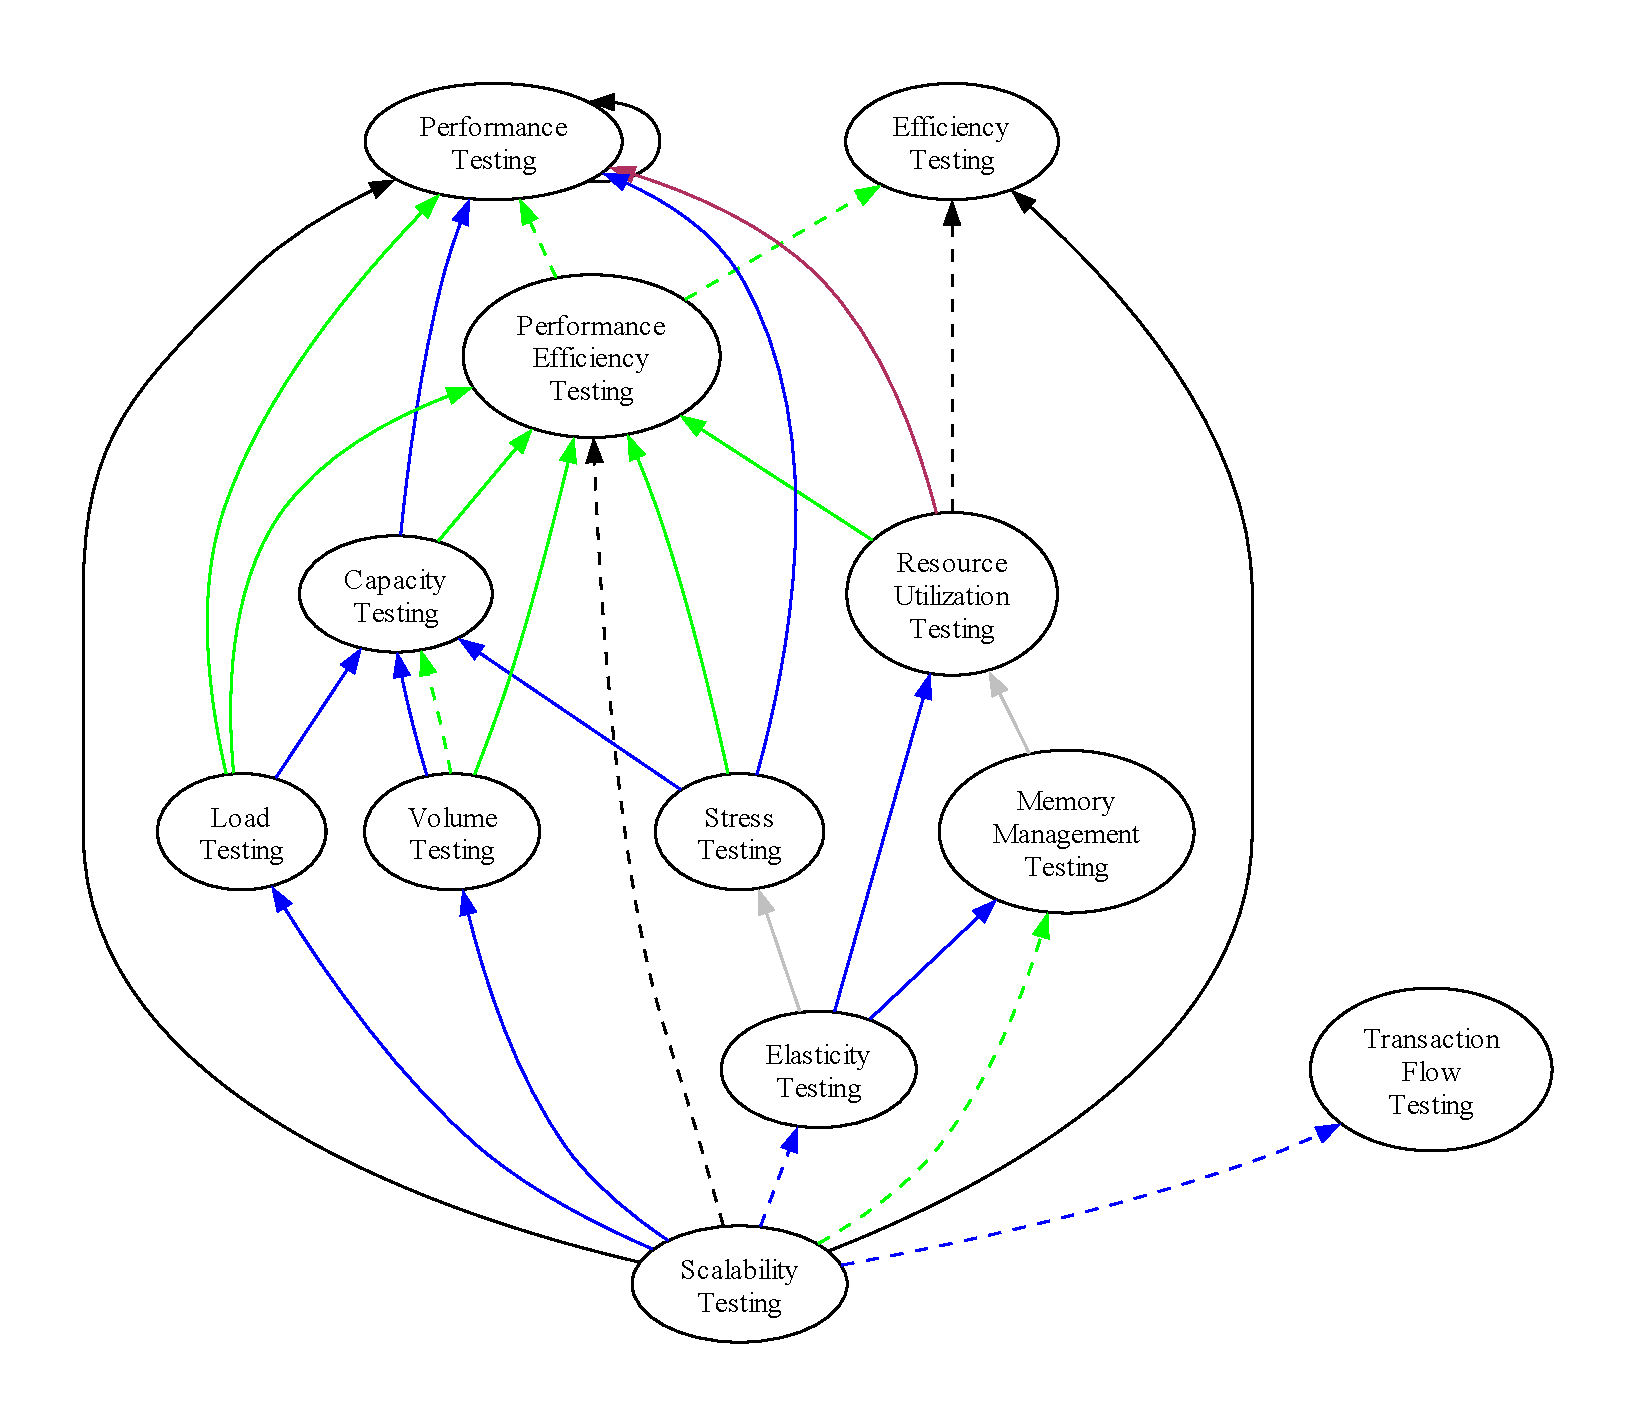
\includegraphics[width=\linewidth]{assets/graphs/scalabilityProposedGraph.pdf}
            \caption{Graph of proposed \ifnotpaper \else \\ \fi relations.}
            \label{fig:scal-graph-proposed}
        \end{subfigure}
        \caption{Graphs of relations between terms related to scalability testing.}
        \label{fig:scalGraphs}
    \end{figure}
}

\newcommand{\performanceGraph}{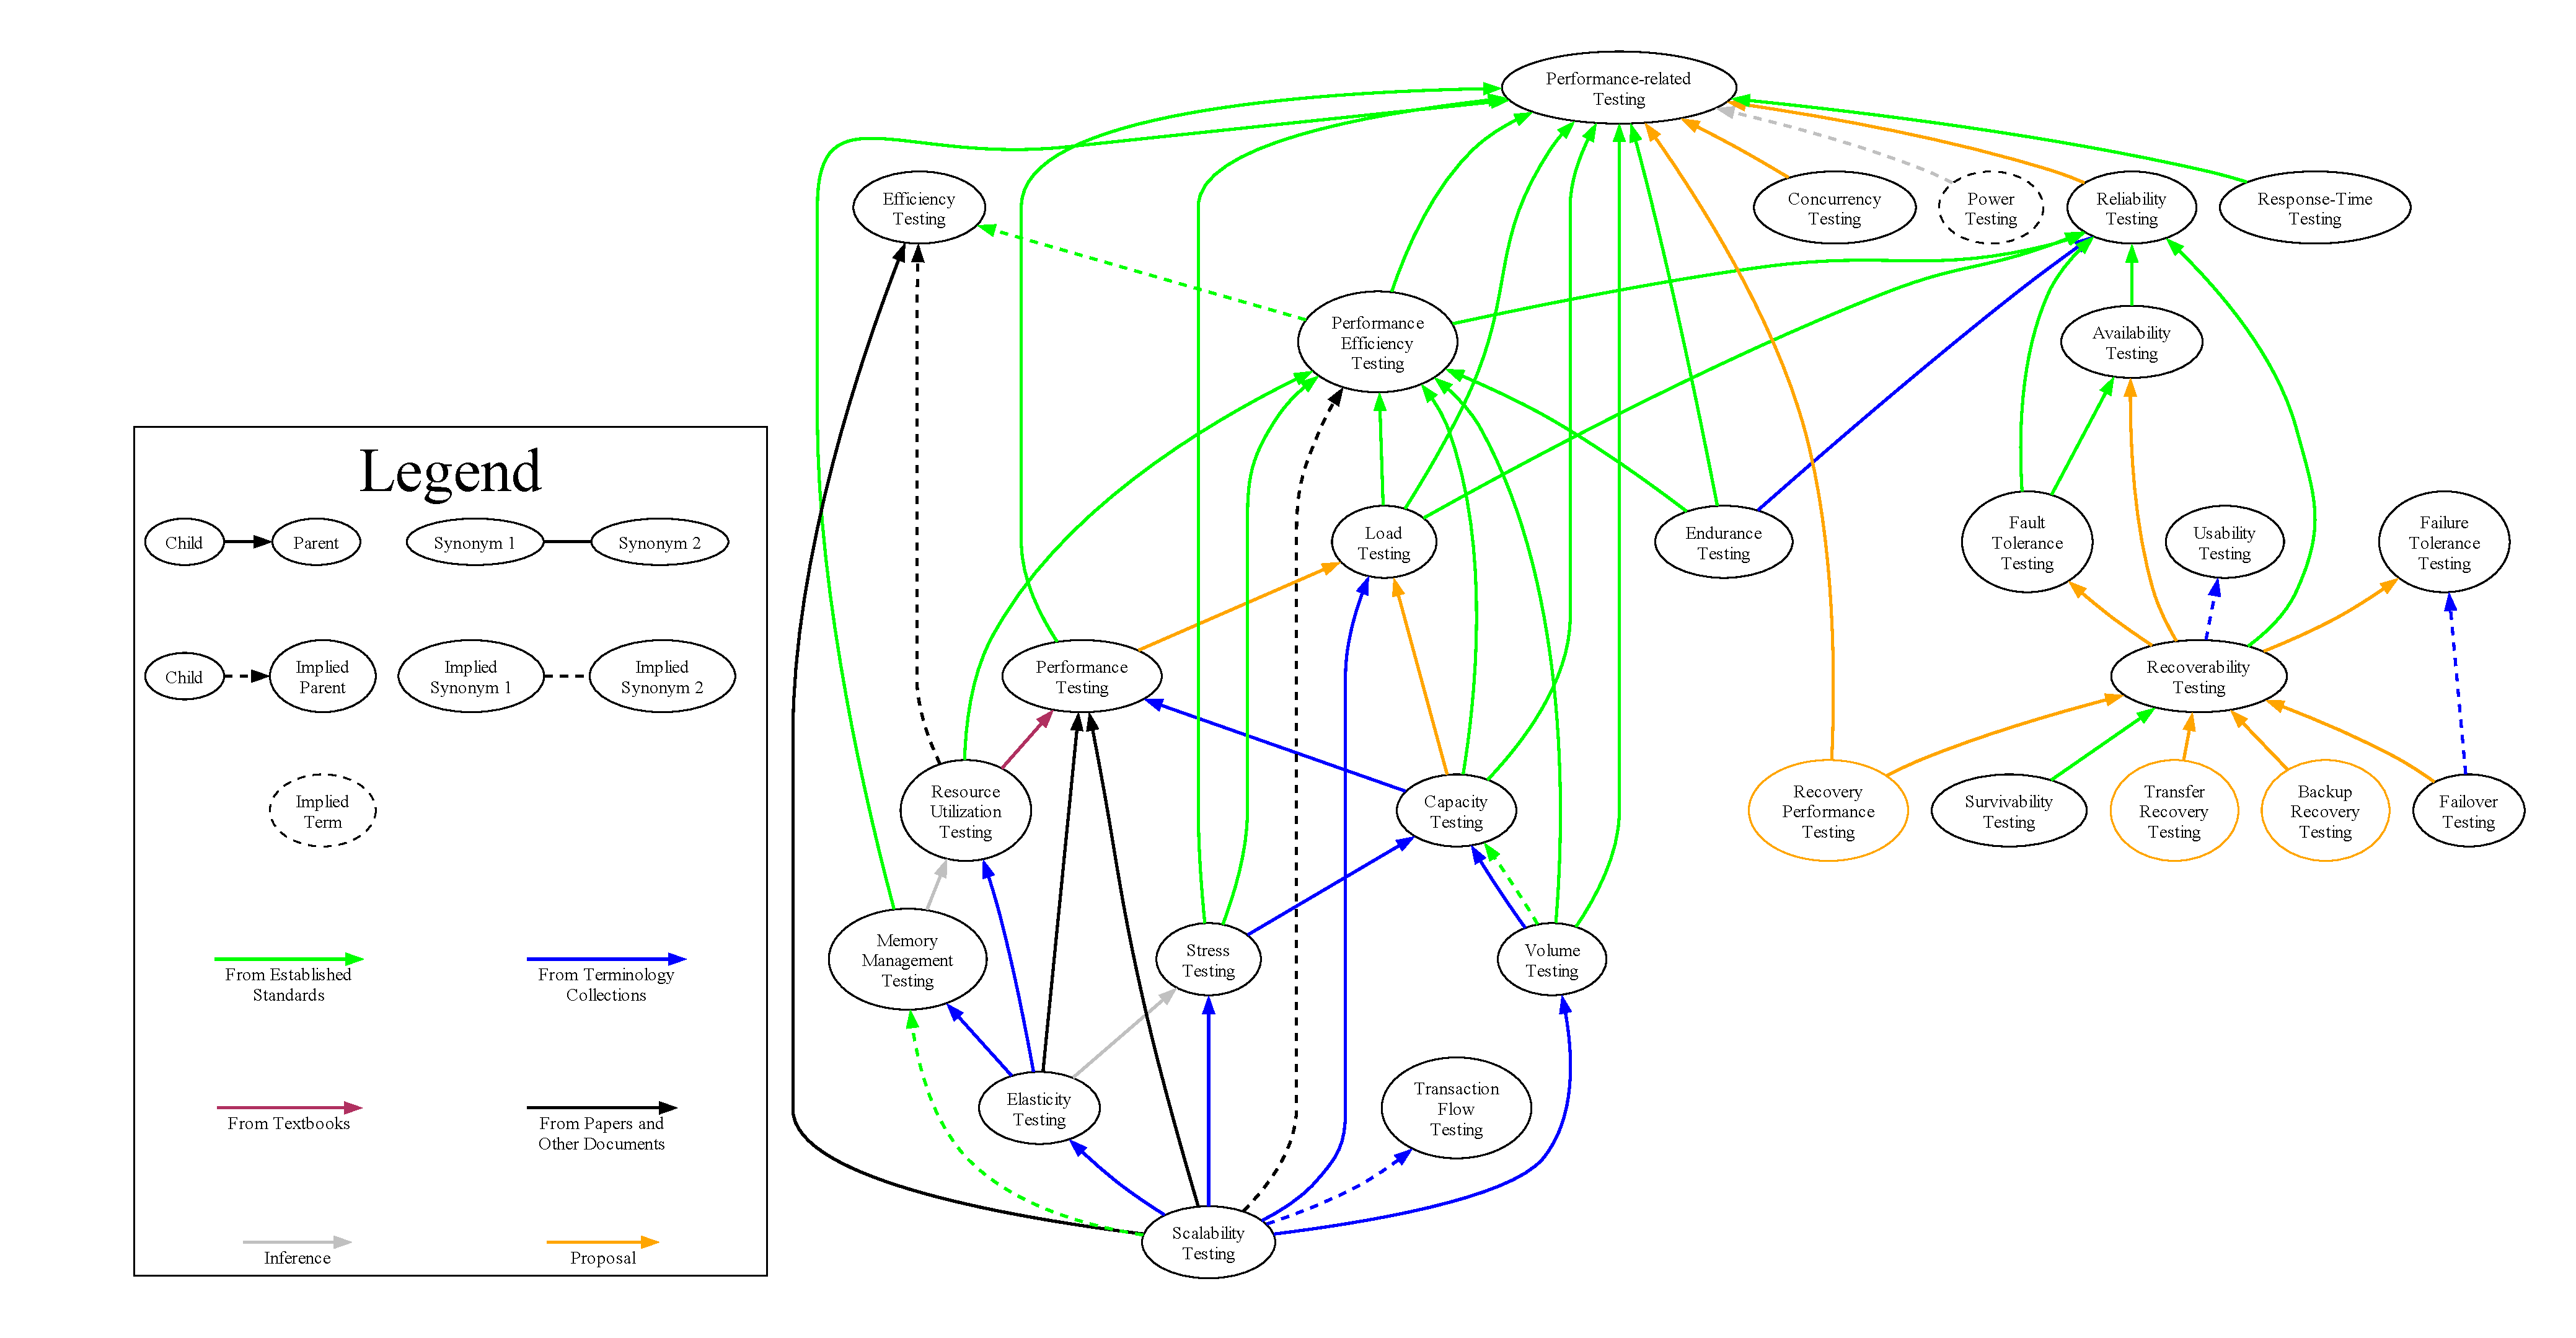
\includegraphics[width=\linewidth]{assets/graphs/performanceProposedGraph.pdf}}

%------------------------------------------------------------------------------
% Images & Figures
%------------------------------------------------------------------------------

\newcommand{\drasilLogo}{assets/images/drasil_logo.png}
\newcommand{\drasilLogoImg}{\input{assets/images/drasil_logo}}
\newcommand{\refDrasilLogoImg}{\Cref{fig:drasilLogo}}

%------------------------------------------------------------------------------
% Tables
%------------------------------------------------------------------------------

% Organization of files
\newcommand{\organizationTable}{\input{assets/tables/organization}}

\newcommand{\ieeeCatsTable}{% Conversion to (longtblr) talltblr assisted by GitHub Copilot

\begin{center}
    \begin{talltblr}[
        note{a} = {Also called ``test phase'' \ifnotpaper (see
                \flawref{level-phase-syns}) \fi or ``test stage'' \ifnotpaper
                (see \flawref{stage-level-syns})\else (see relevant synonym
                flaws in \Cref{syns})\fi.},
        note{b} = {Also called ``test design technique'' \ifnotpaper
                (\citealp[p.~11]{IEEE2022}; \citeyear[p.~5]{IEEE2021a};
                \citealpISTQB{})\else \cite[p.~11]{IEEE2022},
                \cite[p.~5]{IEEE2021a}, \cite{ISTQB}\fi.},
        caption={Categories of test approaches given by ISO/IEC and IEEE.},
        label={tab:ieeeCats}
        ]{
        colspec={|X[0.09,c,m]X[0.575,m]X[0.285,m]|},
        width = \linewidth, rowhead = 1, hlines
        }
        \thead{Term}               & \thead{Definition}                           & \thead{Examples} \\
        Test Level\TblrNote{a}     & A stage of testing ``typically associated
        with the achievement of particular objectives and used to treat particular
        risks'', each performed in sequence \ifnotpaper (\citealp[p.~12]{IEEE2022};
        \citeyear[p.~6]{IEEE2021b}) \else \cite[p.~12]{IEEE2022}, \cite[p.~6]{IEEE2021b}
        \fi with their ``own documentation and resources''
        \citeyearpar[p.~469]{IEEE2017} % ; more generally, ``designat[es] \dots\ the
        % coverage and detail'' \citeyearpar[p.~249]{IEEE2017} 
                                   & unit/component testing, integration testing,
        system testing, acceptance testing \ifnotpaper (\citeyear[p.~12]{IEEE2022};
        \citeyear[p.~6]{IEEE2021b}; \citeyear[p.~467]{IEEE2017}) \else
        \cite[p.~467]{IEEE2017}, \cite[p.~12]{IEEE2022}, \cite[p.~6]{IEEE2021b} \fi                  \\
        Test Practice              & A ``conceptual framework that can be
        applied to \dots{} [a] test process to facilitate testing'' \ifnotpaper
        (\citeyear[p.~14]{IEEE2022}; \citeyear[p.~471]{IEEE2017}; OG IEEE 2013)
        \else \cite[p.~471]{IEEE2017}, \cite[p.~14]{IEEE2022}
        \fi % ; more generally, a ``specific type of activity that contributes to
        % the execution of a process'' \citeyearpar[p.~331]{IEEE2017} 
                                   & scripted testing, exploratory testing,
        automated testing \citeyearpar[p.~20]{IEEE2022}                                              \\
        Test Technique\TblrNote{b} & A ``procedure used to create or select a
        test model \dots, identify test coverage items \dots, and derive
        corresponding test cases'' \ifnotpaper (\citeyear[p.~11]{IEEE2022};
        \citeyear[p.~5]{IEEE2021a}; similar in citeyear[p.~467]{IEEE2017}; OG
        \citeyear{IEEE2013}) \else \cite[p.~11]{IEEE2022}, \cite[p.~5]{IEEE2021a} (similar in
        \cite[p.~467]{IEEE2017}) \fi that ``generate evidence that test item
        requirements have been met or that defects are present in a test item''
        \citeyearpar[p.~vii]{IEEE2021b} ``typically used to achieve a required
        level of coverage'' \citeyearpar[p.~5]{IEEE2021a}
        % ; ``a variety \dots\ is typically
        % required to suitably cover any system'' \citeyearpar[p.~33]{IEEE2022} and
        % is ``often selected based on team skills and familiarity, on the format
        % of the test basis'', and on expectations \citeyearpar[p.~23]{IEEE2022}
                                   & equivalence partitioning,
        boundary value analysis, branch testing \ifnotpaper (\citeyear[p.~11]{IEEE2022};
        \citeyear[p.~5]{IEEE2021a}) \else \cite[p.~11]{IEEE2022}, \cite[p.~5]{IEEE2021a} \fi         \\
        Test Type                  & ``Testing that is focused on specific
        quality characteristics'' \ifnotpaper (\citeyear[p.~15]{IEEE2022};
        \citeyear[p.~7]{IEEE2021b}; \citeyear[p.~473]{IEEE2017}; OG IEEE 2013)
        \else \cite[p.~473]{IEEE2017}, \cite[p.~15]{IEEE2022}, \cite[p.~7]{IEEE2021b}
        \fi                        & security testing, usability testing,
        performance testing \ifnotpaper (\citeyear[p.~15]{IEEE2022};
        \citeyear[p.~8]{IEEE2021a}; \citeyear[p.~473]{IEEE2017}) \else
        \cite[p.~473]{IEEE2017}, \cite[p.~15]{IEEE2022}, \citeyear[p.~8]{IEEE2021a} \fi              \\
    \end{talltblr}
\end{center}
}
\newcommand{\otherCatsTable}{% Defined here so VS Code doesn't freak out
\def\ieeeEquiv{\makecell{IEEE\\Equivalent}}
\def\swebokLevel{{Level\\(objective-\\based)\TblrNote{a}}}

\begin{longtblr}[
    note{a} = {See \flawref{stage-level-syns}.},
    note{b} = {Testing methods and guidances are omitted from this table
            since \citet{BarbosaEtAl2006} do not define or give examples of them.},
    note{c} = {Synonyms for these examples are used by
            \citet[p.~3; OG Mathur, 2012]{SouzaEtAl2017} and
            \citet[p.~3]{BarbosaEtAl2006}.},
    caption={Categories of testing given by other sources.},
    label={tab:otherCats}
    ]{
    colspec={|X[0.08,c,m]|X[0.43,m]|X[0.34,m]|Q[c,m]|},
    width = \linewidth, rowhead = 1
    }
    \hline
    \thead{Term}                           & \thead{Definition}                               & \thead{Examples} & \thead{\ieeeEquiv{}} \\
    \hline
    % Guidance                               & none given
    % \citep[p.~3]{BarbosaEtAl2006}          & none given         & Technique?                              \\
    \swebokLevel{}                         & Test levels based on the
    purpose of testing \citep[p.~5\=/6]{SWEBOK2024} that ``determine
    how the test suite is identified \dots\ regarding its consistency
    \dots\ and its composition''
    \citetext{p.~5\=/2}                    & conformance testing,
    installation testing, regression testing, performance testing,
    security testing % reliability testing,
    \citep[pp.~5\=/7 to 5\=/9]{SWEBOK2024} & Type                                                                                       \\
    % Method                                 & none given
    % \citep[p.~3]{BarbosaEtAl2006}          & none given         & Practice?                               \\
    Phase                                  & none given by \citet{Perry2006} or
    \citet{BarbosaEtAl2006}
    %(\citealp[p.~221]{Perry2006}; \citealp[p.~3]{BarbosaEtAl2006})  
                                           & unit testing,
    integration testing, system testing, regression testing (\citealp[p.~221]{Perry2006};
    \citealp[p.~3]{BarbosaEtAl2006})       & Level                                                                                      \\
    Procedure                              & The basis for how
    testing is performed that guides the process; ``categorized in [to] testing methods,
    testing guidances\TblrNote{b} and testing techniques''
    \citep[p.~3]{BarbosaEtAl2006}          & none given generally by \citet{BarbosaEtAl2006};
    see ``Technique''                      & Approach                                                                                   \\
    Process                                & ``A sequence of
    testing steps'' \citep[p.~2]{BarbosaEtAl2006} ``based on a development technology and \dots\
    paradigm, as well as on a testing procedure''
    \citetext{p.~3}                        & none given by \citet{BarbosaEtAl2006}            & Practice                                \\
    Stage                                  & An
    alternative to the ``traditional \dots\ test stages'' %\footnote{See ``Level'' in \Cref{tab:ieeeCats}.}
    based on ``clear technical groupings''
    \citep[p.~13]{Gerrard2000a}            & desktop development testing,
    infrastructure testing,
    % system testing, large scale integration, and
    post-deployment monitoring
    \citep[p.~13]{Gerrard2000a}            & Level                                                                                      \\
    Technique                              & ``Systematic
    procedures and approaches for generating or selecting the most suitable test suites''
    \citep[p.~5\=/10]{SWEBOK2024}          & specification-based testing,
    % ``on a sound theoretical basis'' \citep[p.~3]{BarbosaEtAl2006}
    structure-based testing, fault-based testing\TblrNote{c}
    % , experience-based testing, usage-based testing
    (\citealp[pp.~5\=/10, 5\=/13 to 5\=/15]{SWEBOK2024})
    % black-box, white-box, defect/fault-based, model-based testing
    % \citetext{\citealp[p.~3]{SouzaEtAl2017}; OG Mathur, 2012};
    % functional, structural, error-based, state-based testing \citep[p.~3]{BarbosaEtAl2006}
                                           & Technique                                                                                  \\
    \hline
\end{longtblr}
}
\newcommand{\otherCategorizationsTable}{\def\visibExs{Specification-based Testing\\ Structure-based Testing\\ Grey-Box Testing}
\def\selecExs{Deterministic Testing\\ Random Testing}
\def\infoSrcExs{Specification-based Testing\\ Structure-based Testing\\
    Experience-based Testing\TblrNote{b}}
\def\apprExs{Specification-based Testing\\ Structure-based Testing\\ (Stepwise) Code Reading}
\def\covCritExs{Input Space Partitioning\\ Graph Coverage\\ Logic Coverage\\ Syntax-based Testing}
\def\questBase{Question Answered: What? When? Where? Who? Why? How? How Well? \citep[p.~17]{Firesmith2015}}
\def\questExs{System Testing\\ Model-based Testing\\ Scenario Testing\TblrNote{C}}
% Pair Testing\\ Unscripted Testing
\def\sdlcExs{Waterfall Testing\\ Incremental Testing\\ \acf{ct}}
\def\reasExs{Smoke Testing\\ Initial Testing\\ Regression Testing}
% Reuse Testing\\ Retesting\\ Error Seeding
\def\execExs{Static Testing\\ Dynamic Testing}
\def\goalExs{Verification Testing\\ Validation Testing}
\def\propExs{Functional Testing\\ Non-functional Testing}
\def\humInvExs{Manual Testing\\ Automated Testing}
\def\humInvCats{Practice \citep[p.~22]{IEEE2022}\\ Technique (see \Cref{tab:multiCats})}
% \citep[implied by][p.~35; see \Cref{tab:multiCats}]{IEEE2022}}
\def\strExs{Scripted Testing\\ Exploratory Testing\TblrNote{f}}
\def\covReqExs{Data Flow Testing\\ Control Flow Testing}
\def\factExs{Correctness Testing\\ Response-Time Testing\\ Access Control Testing\\
    Compliance Testing\\ Reliability Testing\\ Maintainability Testing\\ Portability Testing\\
    Performance Testing\TblrNote{e}}
\def\dataSrcExs{Specification-based Testing\\ Implementation-oriented Testing\\ Error-oriented Testing}
\def\adqCritExs{Coverage-based Testing\\ Fault-based Testing\\ Error-based Testing}
\def\typeCatExs{Static Testing\\ Test Browsing\\ Functional Testing\\
    Non-functional Testing\\ Large Scale Integration (Testing)}
\def\priorExs{Smoke Testing\\ Usability Testing\\ Performance Testing\\ Functionality Testing}
\def\purpExs{Correctness Testing\\ Performance Testing\\ Reliability Testing\\ Security Testing}

\newcommand\firesmithSubset[1]{\citep[p.~#1]{Firesmith2015}\TblrNote{d}}

\begin{longtblr}[
    note{a} = {Defined in \Cref{par-chd-rels}.},
    note{b} = {\citet[p.~440]{PetersAndPedrycz2000} replace the latter two with
            ``implementation-oriented testing'' and ``error-oriented testing''.},
    note{c} = {Experience-based testing may instead be a ``practice'' (see \Cref{tab:multiCats}).},
    % note{C} = {This list is \emph{quite} nonexhaustive.},
    note{d} = {We only present a subset of the test bases and example approaches from
            \citep{Firesmith2015} for brevity.},
    note{e} = {We also consider this categorization meaningful (see \Cref{static-test}).},
    % note{e} = {Other test factors are given that do not unambiguously map to corresponding
    %         test approaches: file integrity, authorization, audit trail, continuity of processing,
    %         service levels, ease of use, coupling (e.g., with other applications in a given environment),
    %         and ease of operation (e.g., documentation, training) \citep[pp.~40--41]{Perry2006}.},
    note{f} = {This grouping is likely incorrect (see \Cref{exp-unscrip}).},
    note{g} = {Exploratory testing may instead be a ``technique'' (see \Cref{tab:multiCats}).},
    note{h} = {\citet[p.~49]{Firesmith2015} less-than-helpfully calls this basis ``whitebox testing''.},
    note{i} = \gerrardDistinctIEEE*{type},
    note{j} = {With the exception of smoke testing, which is categorized as a technique
            (\citealp[p.~5\=/14]{SWEBOK2024}; \citealp[pp.~601, 603, 605--606]{SharmaEtAl2021});
            performance testing is also sometimes categorized as a technique \citep[p.~38]{IEEE2021}.},
    caption = {Alternate categorizations found in the literature.},
    label = {tab:otherCategorizations}
    ]{
    colspec = {|X[0.375,c,m]X[0.275,c,m]X[0.35,c,m]|},
    width = \linewidth, rowhead = 1
    }
    \hline
    \thead{Test Basis}                      & \thead{Example Approaches} & \thead{Parent\TblrNote{a} IEEE Category}                                                                                                 \\
    \hline
    Visibility of the \acs{sut}'s Internal Structure (\citealp[p.~8]{IEEE2021};
    \citealp[pp.~5\=/10, 5\=/16]{SWEBOK2024};
    % \citealp[pp.~53, 218]{Patton2006}; \citealp[p.~69]{Perry2006}; \citealp[p.~601; OG {[8]}]{SharmaEtAl2021};
    % \citealp[pp.~57--58]{AmmannAndOffutt2017}; \citealp[p.~213]{KuļešovsEtAl2013}; \citep[pp.~4--5]{Kam2008}
    six other sources)                      & \visibExs{}                & Technique (\citealp[pp.~4, 8]{IEEE2021}; \citealp[p.~46]{Firesmith2015})                                                                 \\
    \hline
    Source of Information for Designing Tests
    \citep[p.~8; one more source]{IEEE2021} & \infoSrcExs{}              & Technique\TblrNote{c} (\citealp[p.~22]{IEEE2022}; \citeyear[p.~4]{IEEE2021}; three other sources)                                        \\
    % & & \citealp[pp.~5\=/10, 5\=/13]{SWEBOK2024}; \citealpISTQB{}; \citealp[p.~46]{Firesmith2015}) \\
    \hline
    % Source of Test Data
    % \citep[p.~440]{PetersAndPedrycz2000}    & \dataSrcExs{}              & Technique                                                                                                                                \\
    % \hline
    Selection Process
    \citep[p.~5-16]{SWEBOK2024}             & \selecExs{}                & Technique \citep[pp.~5\=/12, 5\=/16]{SWEBOK2024}                                                                                         \\
    \hline
    % \questBase{}                             & \questExs{}                & Approach                                                                                                                                                               \\
    % \hline
    Stage of Lifecycle \firesmithSubset{29} & \sdlcExs{}                 & Practice                                                                                                                                 \\
    \hline
    Reason \firesmithSubset{34}             & \reasExs{}                 & Technique                                                                                                                                \\
    \hline
    Level of Automation \firesmithSubset{44;
        % \citep[p.~214]{KuļešovsEtAl2013}
    one other source}                       & \humInvExs{}               & \humInvCats{}                                                                                                                            \\
    \hline
    Execution of Code\TblrNote{e} \citep[p.~53; two other sources]{Patton2006}
    % \citealp[p.~214]{KuļešovsEtAl2013}; \citealp[p.~12]{Gerrard2000a}
                                            & \execExs{}                 & Approach                                                                                                                                 \\
    \hline
    Goal \citep[pp.~69--70; one other source]{Perry2006};
    % \citealp[p.~214]{KuļešovsEtAl2013}
                                            & \goalExs{}                 & Approach                                                                                                                                 \\
    \hline
    % Seems synonymous with testing based on software qualities
    % Test Factor (also called Quality Factor or Quality Attribute)
    % \citep[pp.~40--41]{Perry2006}           & \factExs{}                 & Type (\citealp[p.~22]{IEEE2022}; and/or implied by its quality and/or \citealp{Firesmith2015})                                           \\
    % \hline
    Adequacy Criterion
    \citep[pp.~398--399]{vanVliet2000}      & \adqCritExs{}              & Technique \citep[pp.~398--399]{vanVliet2000}                                                                                             \\
    \hline
    Coverage Criteria
    \citep[pp.~18--19]{AmmannAndOffutt2017} & \covCritExs{}              & Technique (\citealp[p.~22]{IEEE2022}; \citeyear[Fig.~2]{IEEE2021}; \citealp[p.~5\=/11]{SWEBOK2024}; \citealp[pp.~47--48]{Firesmith2015}) \\
    \hline
    Structuredness
    \citep[p.~214]{KuļešovsEtAl2013}        & \strExs{}                  & Practice\TblrNote{g} \citep[pp.~20, 22]{IEEE2022}                                                                                        \\
    \hline
    Property of Code \citep[p.~213]{KuļešovsEtAl2013}
    or Test Target
    \citep[pp.~4--5]{Kam2008}               & \propExs{}                 & Ambiguous (see \Cref{func-test-flaw})                                                                                                    \\
    \hline
    Coverage Requirement\TblrNote{h}
    \citep[pp.~4--5]{Kam2008}               & \covReqExs{}               & Technique (\citealp[p.~5\=/13]{SWEBOK2024}; \citealp[p.~49]{Firesmith2015})                                                              \\
    \hline
    Category of Test Type\TblrNote{i}
    \citep[p.~12]{Gerrard2000a}             & \typeCatExs{}              & Ambiguous                                                                                                                                \\
    \hline
    Priority (in the context of testing e-business projects)
    \citep[p.~13]{Gerrard2000a}             & \priorExs{}                & Type\TblrNote{j} (\citealp[p.~22]{IEEE2022}; \citeyear[Tab.~A.1]{IEEE2021}; and/or implied by \citealp[p.~53]{Firesmith2015})            \\
    \hline
    Purpose \citep{Pan1999}                 & \purpExs{}                 & Type (\citealp[p.~22]{IEEE2022}; and/or implied by \citealp[p.~53]{Firesmith2015})                                                       \\
    \hline
\end{longtblr}
}

\newcommand{\flawMnfstsTable}{\begin{paperTable}
    \centering
    \caption{Breakdown of identified \nameref{flawMnfsts} by \srcCat{}.}
    \label{tab:flawMnfsts}
    \begin{minipage}{\linewidth}
        \begin{tabular}{|r|*{6}{cc|}c|}
            \hline
                              & \multicolumn{2}{c|}{\thead{\wrong{}}} & \multicolumn{2}{c|}{\thead{\miss{}}} & \multicolumn{2}{c|}{\thead{\contra{}}} & \multicolumn{2}{c|}{\thead{\ambi{}}} & \multicolumn{2}{c|}{\thead{\over{}}} & \multicolumn{2}{c|}{\thead{\redun{}}} &                                                                                                                                                                                                \\
            \thead{\srcCat{}} & \thead{Exp}                           & \thead{Imp}                          & \thead{Exp}                            & \thead{Imp}                          & \thead{Exp}                          & \thead{Imp}                           & \thead{Exp}              & \thead{Imp}              & \thead{Exp}              & \thead{Imp}               & \thead{Exp}               & \thead{Imp}               & \thead{Total}             \\
            \hline
            \stds{}           & \stdFlawMnfstBrkdwn{1}                & \stdFlawMnfstBrkdwn{2}               & \stdFlawMnfstBrkdwn{3}                 & \stdFlawMnfstBrkdwn{4}               & \stdFlawMnfstBrkdwn{5}               & \stdFlawMnfstBrkdwn{6}                & \stdFlawMnfstBrkdwn{7}   & \stdFlawMnfstBrkdwn{8}   & \stdFlawMnfstBrkdwn{9}   & \stdFlawMnfstBrkdwn{10}   & \stdFlawMnfstBrkdwn{11}   & \stdFlawMnfstBrkdwn{12}   & \stdFlawMnfstBrkdwn{13}   \\
            \metas{}          & \metaFlawMnfstBrkdwn{1}               & \metaFlawMnfstBrkdwn{2}              & \metaFlawMnfstBrkdwn{3}                & \metaFlawMnfstBrkdwn{4}              & \metaFlawMnfstBrkdwn{5}              & \metaFlawMnfstBrkdwn{6}               & \metaFlawMnfstBrkdwn{7}  & \metaFlawMnfstBrkdwn{8}  & \metaFlawMnfstBrkdwn{9}  & \metaFlawMnfstBrkdwn{10}  & \metaFlawMnfstBrkdwn{11}  & \metaFlawMnfstBrkdwn{12}  & \metaFlawMnfstBrkdwn{13}  \\
            \texts{}          & \textFlawMnfstBrkdwn{1}               & \textFlawMnfstBrkdwn{2}              & \textFlawMnfstBrkdwn{3}                & \textFlawMnfstBrkdwn{4}              & \textFlawMnfstBrkdwn{5}              & \textFlawMnfstBrkdwn{6}               & \textFlawMnfstBrkdwn{7}  & \textFlawMnfstBrkdwn{8}  & \textFlawMnfstBrkdwn{9}  & \textFlawMnfstBrkdwn{10}  & \textFlawMnfstBrkdwn{11}  & \textFlawMnfstBrkdwn{12}  & \textFlawMnfstBrkdwn{13}  \\
            \papers*{}        & \paperFlawMnfstBrkdwn{1}              & \paperFlawMnfstBrkdwn{2}             & \paperFlawMnfstBrkdwn{3}               & \paperFlawMnfstBrkdwn{4}             & \paperFlawMnfstBrkdwn{5}             & \paperFlawMnfstBrkdwn{6}              & \paperFlawMnfstBrkdwn{7} & \paperFlawMnfstBrkdwn{8} & \paperFlawMnfstBrkdwn{9} & \paperFlawMnfstBrkdwn{10} & \paperFlawMnfstBrkdwn{11} & \paperFlawMnfstBrkdwn{12} & \paperFlawMnfstBrkdwn{13} \\
            \hline
            Total             & \totalFlawMnfstBrkdwn{1}              & \totalFlawMnfstBrkdwn{2}             & \totalFlawMnfstBrkdwn{3}               & \totalFlawMnfstBrkdwn{4}             & \totalFlawMnfstBrkdwn{5}             & \totalFlawMnfstBrkdwn{6}              & \totalFlawMnfstBrkdwn{7} & \totalFlawMnfstBrkdwn{8} & \totalFlawMnfstBrkdwn{9} & \totalFlawMnfstBrkdwn{10} & \totalFlawMnfstBrkdwn{11} & \totalFlawMnfstBrkdwn{12} & \totalFlawMnfstBrkdwn{13} \\
            \hline
        \end{tabular}
    \end{minipage}
\end{paperTable}
}
\newcommand{\flawDmnsTable}{\begin{paperTable}
    \centering
    \caption{Breakdown of identified \nameref{flawDmns} by \srcCat{}.}
    \label{tab:flawDmns}
    % \begin{minipage}{\linewidth}
    \begin{tabular}{|r|*{6}{cc|}c|}
        \hline
                          & \multicolumn{2}{c|}{\thead{\cats{}}} & \multicolumn{2}{c|}{\thead{\syns{}}} & \multicolumn{2}{c|}{\thead{\pars{}}} & \multicolumn{2}{c|}{\thead{\defs{}}} & \multicolumn{2}{c|}{\thead{\terms{}}} & \multicolumn{2}{c|}{\thead{\cites{}}} &                                                                                                                                                                                  \\
        % \cline{2-10}
        \thead{\srcCat{}} & \thead{Exp}                          & \thead{Imp}                          & \thead{Exp}                          & \thead{Imp}                          & \thead{Exp}                           & \thead{Imp}                           & \thead{Exp}            & \thead{Imp}            & \thead{Exp}            & \thead{Imp}             & \thead{Exp}             & \thead{Imp}             & \thead{Total}           \\
        \hline
        \stds{}           & \stdFlawDmnBrkdwn{1}                 & \stdFlawDmnBrkdwn{2}                 & \stdFlawDmnBrkdwn{3}                 & \stdFlawDmnBrkdwn{4}                 & \stdFlawDmnBrkdwn{5}                  & \stdFlawDmnBrkdwn{6}                  & \stdFlawDmnBrkdwn{7}   & \stdFlawDmnBrkdwn{8}   & \stdFlawDmnBrkdwn{9}   & \stdFlawDmnBrkdwn{10}   & \stdFlawDmnBrkdwn{11}   & \stdFlawDmnBrkdwn{12}   & \stdFlawDmnBrkdwn{13}   \\
        \metas{}          & \metaFlawDmnBrkdwn{1}                & \metaFlawDmnBrkdwn{2}                & \metaFlawDmnBrkdwn{3}                & \metaFlawDmnBrkdwn{4}                & \metaFlawDmnBrkdwn{5}                 & \metaFlawDmnBrkdwn{6}                 & \metaFlawDmnBrkdwn{7}  & \metaFlawDmnBrkdwn{8}  & \metaFlawDmnBrkdwn{9}  & \metaFlawDmnBrkdwn{10}  & \metaFlawDmnBrkdwn{11}  & \metaFlawDmnBrkdwn{12}  & \metaFlawDmnBrkdwn{13}  \\
        \texts{}          & \textFlawDmnBrkdwn{1}                & \textFlawDmnBrkdwn{2}                & \textFlawDmnBrkdwn{3}                & \textFlawDmnBrkdwn{4}                & \textFlawDmnBrkdwn{5}                 & \textFlawDmnBrkdwn{6}                 & \textFlawDmnBrkdwn{7}  & \textFlawDmnBrkdwn{8}  & \textFlawDmnBrkdwn{9}  & \textFlawDmnBrkdwn{10}  & \textFlawDmnBrkdwn{11}  & \textFlawDmnBrkdwn{12}  & \textFlawDmnBrkdwn{13}  \\
        \papersTbl{}      & \paperFlawDmnBrkdwn{1}               & \paperFlawDmnBrkdwn{2}               & \paperFlawDmnBrkdwn{3}               & \paperFlawDmnBrkdwn{4}               & \paperFlawDmnBrkdwn{5}                & \paperFlawDmnBrkdwn{6}                & \paperFlawDmnBrkdwn{7} & \paperFlawDmnBrkdwn{8} & \paperFlawDmnBrkdwn{9} & \paperFlawDmnBrkdwn{10} & \paperFlawDmnBrkdwn{11} & \paperFlawDmnBrkdwn{12} & \paperFlawDmnBrkdwn{13} \\
        \hline
        Total             & \totalFlawDmnBrkdwn{1}               & \totalFlawDmnBrkdwn{2}               & \totalFlawDmnBrkdwn{3}               & \totalFlawDmnBrkdwn{4}               & \totalFlawDmnBrkdwn{5}                & \totalFlawDmnBrkdwn{6}                & \totalFlawDmnBrkdwn{7} & \totalFlawDmnBrkdwn{8} & \totalFlawDmnBrkdwn{9} & \totalFlawDmnBrkdwn{10} & \totalFlawDmnBrkdwn{11} & \totalFlawDmnBrkdwn{12} & \totalFlawDmnBrkdwn{13} \\
        \hline
    \end{tabular}
    % \end{minipage}
\end{paperTable}}

\newcommand{\testReqsTable}{\input{assets/tables/testReqs}}
